\documentclass[border=6pt,tikz]{standalone}
\usepackage{tikz}
\usepackage{amsmath,amssymb}
\usetikzlibrary{arrows.meta,positioning,fit,backgrounds,calc,shapes.geometric,decorations.pathreplacing,patterns}
\definecolor{ink}{HTML}{1B2430}
\definecolor{muted}{HTML}{6B7785}
\definecolor{accent}{HTML}{2F6FB5}
\definecolor{accent2}{HTML}{C1611F}
\definecolor{good}{HTML}{2E7D5B}
\definecolor{soft}{HTML}{EDF2F7}
\definecolor{soft2}{HTML}{FBEDE2}
\definecolor{soft3}{HTML}{E6F0E9}
\tikzset{
  box/.style={draw=ink,line width=.7pt,rounded corners=2pt,fill=soft,inner sep=4pt,align=center,font=\sffamily\small},
  boxa/.style={box,fill=soft2},
  boxb/.style={box,fill=soft3},
  plain/.style={align=center,font=\sffamily\small,text=ink},
  tiny/.style={align=center,font=\sffamily\scriptsize,text=muted},
  ar/.style={-{Stealth[length=2.4mm]},draw=ink,line width=.7pt},
  arm/.style={-{Stealth[length=2.4mm]},draw=muted,line width=.6pt,dashed},
  nd/.style={circle,draw=ink,line width=.7pt,fill=white,minimum size=7mm,inner sep=0pt,font=\sffamily\scriptsize},
  ndf/.style={nd,fill=soft},
  ndt/.style={nd,fill=soft2},
}

\begin{document}
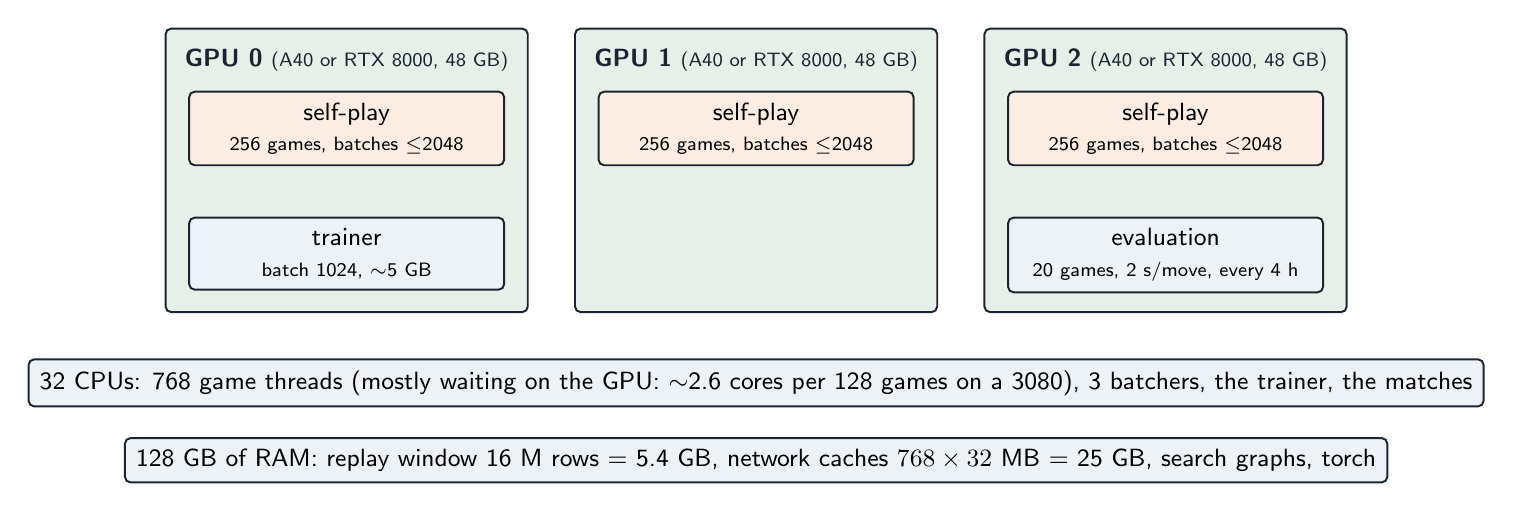
\begin{tikzpicture}[x=1mm,y=1mm]
  \foreach \g/\x in {0/0,1/52,2/104} {
    \node[boxb,minimum width=46mm,minimum height=36mm,anchor=north] (g\g) at (\x,0) {};
    \node[plain,anchor=north] at (\x,-1.5) {\textbf{GPU \g}\ \scriptsize(A40 or RTX 8000, 48 GB)};
    \node[boxa,minimum width=40mm,anchor=north] (s\g) at (\x,-8) {self-play\\\scriptsize 256 games, batches $\le$2048};
  }
  \node[box,minimum width=40mm,anchor=north] at (0,-24) {trainer\\\scriptsize batch 1024, $\sim$5 GB};
  \node[box,minimum width=40mm,anchor=north] at (104,-24) {evaluation\\\scriptsize 20 games, 2 s/move, every 4 h};
  \node[box,minimum width=150mm,anchor=north] (cpu) at (52,-42) {32 CPUs: 768 game threads (mostly waiting on the GPU: $\sim$2.6 cores per 128 games on a 3080), 3 batchers, the trainer, the matches};
  \node[box,minimum width=150mm,anchor=north] (ram) at (52,-52) {128 GB of RAM: replay window 16 M rows = 5.4 GB, network caches $768\times32$ MB = 25 GB, search graphs, torch};
\end{tikzpicture}
\end{document}
